% =====================================================================
%  preamble.tex —— 河野俊丈《場の理論とトポロジー》中文译注本 · 导言区
%  Lead 独占；译者只读，不得修改
% =====================================================================
\usepackage[b5paper,top=21mm,bottom=21mm,left=19mm,right=19mm,headsep=5mm,footskip=9mm]{geometry}
\usepackage{amsmath,amssymb,mathrsfs,bm}
\usepackage{graphicx}
\usepackage{xcolor}
\usepackage{booktabs,array,multirow,longtable,multicol}
\usepackage{enumitem}
\usepackage{fancyhdr}
\usepackage{caption}
\usepackage{tcolorbox}
\tcbuselibrary{most}
\usepackage{tikz}
\usepackage{hyperref}
\hypersetup{colorlinks=true,linkcolor=black,citecolor=black,urlcolor=blue!45!black,
            bookmarksnumbered=true,pdftitle={场论与拓扑学（河野俊丈 著，中文译注本）},
            pdfauthor={河野俊丈 著}}

\setlength{\parindent}{2em}
\linespread{1.12}
\allowdisplaybreaks[2]
\setlength{\emergencystretch}{6em}
\tolerance=3000
\hbadness=10000

% ---------- 页眉页脚 ----------
\pagestyle{fancy}
\fancyhf{}
\renewcommand{\headrulewidth}{0.3pt}
\fancyhead[LE]{\small\thepage}
\fancyhead[RE]{\small\leftmark}
\fancyhead[RO]{\small\thepage}
\fancyhead[LO]{\small\rightmark}
\fancyfoot{}
\renewcommand{\chaptermark}[1]{\markboth{\CTEXthechapter\quad #1}{}}
\renewcommand{\sectionmark}[1]{\markright{\thesection\quad #1}}

% ---------- 章节标题格式 ----------
\ctexset{
  chapter = {
    format = \centering\Large\bfseries,
    name = {第,章},
    number = \arabic{chapter},
    beforeskip = 18pt,
    afterskip = 22pt,
  },
  section = {
    format = \large\bfseries,
    beforeskip = 14pt,
    afterskip = 10pt,
  },
  subsection = {
    format = \normalsize\bfseries,
    beforeskip = 11pt,
    afterskip = 6pt,
  },
}

% ---------- 公式编号：章.序号（原书同此制；实际一律 \tag 手工给号）----------
\numberwithin{equation}{chapter}

% ---------- 陈述环境：编号一律由原文抄录（手工），不使用自动计数器 ----------
% 用法：\begin{definition}{1.3} …… \end{definition}
\newcommand{\fkstmt}[2]{\par\medskip\noindent\textbf{#1~#2}\ \ignorespaces}
\newenvironment{definition}[1]{\fkstmt{定义}{#1}}{\hfill$\square$\par\medskip}
% 定理/引理/命题/推论：带 * 版用于「后面紧跟证明」的陈述（原书无 □）；不带 * 版补 □
\newenvironment{theorem}[1]{\fkstmt{定理}{#1}}{\hfill$\square$\par\medskip}
\newenvironment{theorem*}[1]{\fkstmt{定理}{#1}}{\par\medskip}
\newenvironment{lemma}[1]{\fkstmt{引理}{#1}}{\hfill$\square$\par\medskip}
\newenvironment{lemma*}[1]{\fkstmt{引理}{#1}}{\par\medskip}
\newenvironment{proposition}[1]{\fkstmt{命题}{#1}}{\hfill$\square$\par\medskip}
\newenvironment{proposition*}[1]{\fkstmt{命题}{#1}}{\par\medskip}
\newenvironment{corollary}[1]{\fkstmt{推论}{#1}}{\hfill$\square$\par\medskip}
\newenvironment{corollary*}[1]{\fkstmt{推论}{#1}}{\par\medskip}
\newenvironment{example}[1]{\fkstmt{例}{#1}}{\hfill$\square$\par\medskip}
\newenvironment{remark}[1]{\fkstmt{注}{#1}}{\par\medskip}
\newenvironment{question}[1]{\fkstmt{问}{#1}}{\par\medskip}
\newenvironment{problem}[1]{\fkstmt{问题}{#1}}{\par\medskip}
\newenvironment{conjecture}[1]{\fkstmt{猜想}{#1}}{\par\medskip}
\newenvironment{counterexample}[1]{\fkstmt{反例}{#1}}{\par\medskip}
\newenvironment{notation}[1]{\fkstmt{记号}{#1}}{\par\medskip}
\newenvironment{assumption}[1]{\fkstmt{假设}{#1}}{\hfill$\square$\par\medskip}
\newenvironment{formulaenv}[1]{\fkstmt{公式}{#1}}{\par\medskip}
\newenvironment{proof}[1][证明]{\par\medskip\noindent\textbf{#1}\ \ignorespaces}{\hfill$\blacksquare$\par\medskip}

% ---------- 行内小标题（原书 \textbf{...} 独立成段）----------
\newcommand{\para}[1]{\par\medskip\noindent\textbf{#1}\ \ignorespaces}

% ---------- 图题（手工编号，与原书一致）----------
\newcommand{\figtitle}[2]{\par\smallskip\noindent{\centering\small 图~#1\quad #2\par}\smallskip}
% 用法：\begin{figure}[htbp]\centering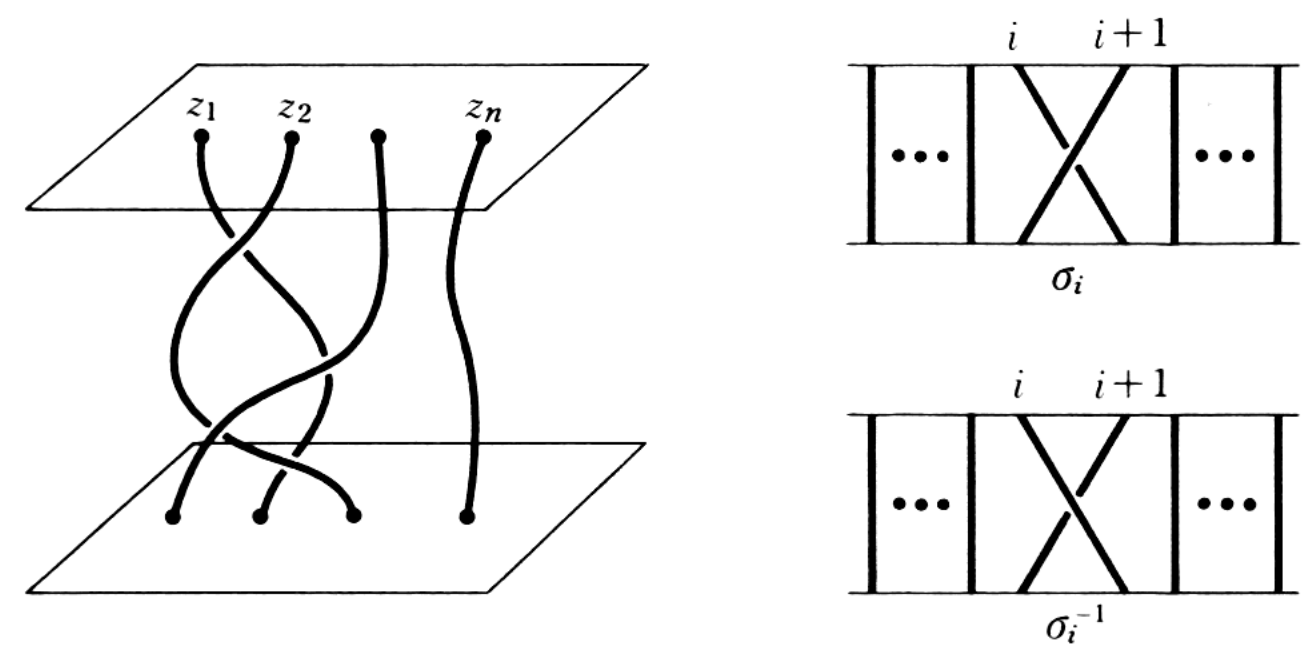
\includegraphics[width=.6\textwidth]{figures/fig2.1.png}\figtitle{2.1}{……（原书 p.41）}\end{figure}

% ---------- 表题 ----------
\newcommand{\tabtitle}[2]{\par\smallskip\noindent{\centering\small 表~#1\quad #2\par}\smallskip}

% ---------- “本节重点” 与 “章末评注”（全局开关）----------
\newif\ifshowtakeaway     \showtakeawaytrue
\newif\ifshowchapterreview \showchapterreviewtrue

\newtcolorbox{takeawaybox}{
  enhanced, breakable, colback=blue!4!white, colframe=blue!55!black,
  boxrule=0.4pt, arc=1.5pt, left=5pt, right=5pt, top=3pt, bottom=3pt,
  title={\small\bfseries 本节重点}, fonttitle=\small\bfseries,
  coltitle=white, colbacktitle=blue!55!black, attach boxed title to top left={xshift=4pt,yshift=-2pt},
}
\newtcolorbox{reviewbox}{
  enhanced, breakable, colback=orange!3!white, colframe=orange!65!black,
  boxrule=0.4pt, arc=1.5pt, left=6pt, right=6pt, top=4pt, bottom=4pt,
  title={\small\bfseries 本章回顾与评注}, fonttitle=\small\bfseries,
  coltitle=white, colbacktitle=orange!65!black, attach boxed title to top left={xshift=4pt,yshift=-2pt},
}
\newcommand{\takeaway}[1]{\ifshowtakeaway\begin{takeawaybox}\small #1\end{takeawaybox}\fi}
\newcommand{\chapterreview}[1]{\ifshowchapterreview\begin{reviewbox}\small #1\end{reviewbox}\fi}

% ---------- 常用记号 ----------
\newcommand{\R}{\mathbb{R}}
\newcommand{\C}{\mathbb{C}}
\newcommand{\Z}{\mathbb{Z}}
\newcommand{\Q}{\mathbb{Q}}
\newcommand{\N}{\mathbb{N}}
\newcommand{\HH}{\mathbb{H}}
\newcommand{\RP}{\mathbb{R}P}
\newcommand{\CP}{\mathbb{C}P}
\newcommand{\T}{\mathbb{T}}
\newcommand{\rd}{\mathrm{d}}
\newcommand{\id}{\mathrm{id}}
\newcommand{\cA}{\mathcal{A}}
\newcommand{\cB}{\mathcal{B}}
\newcommand{\cC}{\mathcal{C}}
\newcommand{\cD}{\mathcal{D}}
\newcommand{\cE}{\mathcal{E}}
\newcommand{\cF}{\mathcal{F}}
\newcommand{\cG}{\mathcal{G}}
\newcommand{\cH}{\mathcal{H}}
\newcommand{\cI}{\mathcal{I}}
\newcommand{\cJ}{\mathcal{J}}
\newcommand{\cK}{\mathcal{K}}
\newcommand{\cL}{\mathcal{L}}
\newcommand{\cM}{\mathcal{M}}
\newcommand{\cN}{\mathcal{N}}
\newcommand{\cO}{\mathcal{O}}
\newcommand{\cP}{\mathcal{P}}
\newcommand{\cQ}{\mathcal{Q}}
\newcommand{\cR}{\mathcal{R}}
\newcommand{\cS}{\mathcal{S}}
\newcommand{\cT}{\mathcal{T}}
\newcommand{\cU}{\mathcal{U}}
\newcommand{\cV}{\mathcal{V}}
\newcommand{\cW}{\mathcal{W}}
\newcommand{\cX}{\mathcal{X}}
\newcommand{\cY}{\mathcal{Y}}
\newcommand{\cZ}{\mathcal{Z}}
\newcommand{\fA}{\mathfrak{a}}
\newcommand{\fg}{\mathfrak{g}}
\newcommand{\fh}{\mathfrak{h}}
\newcommand{\fn}{\mathfrak{n}}
\newcommand{\fsl}{\mathfrak{sl}}
\newcommand{\fsu}{\mathfrak{su}}
\newcommand{\fso}{\mathfrak{so}}
\newcommand{\fgl}{\mathfrak{gl}}
% 常用算子（正体）
\newcommand{\Tr}{\operatorname{Tr}}
\newcommand{\tr}{\operatorname{tr}}
\newcommand{\End}{\operatorname{End}}
\newcommand{\Hom}{\operatorname{Hom}}
\newcommand{\Aut}{\operatorname{Aut}}
\newcommand{\Diff}{\operatorname{Diff}}
\newcommand{\Map}{\operatorname{Map}}
\newcommand{\Conf}{\operatorname{Conf}}
\newcommand{\Rep}{\operatorname{Rep}}
\newcommand{\Res}{\operatorname{Res}}
\newcommand{\Ind}{\operatorname{Ind}}
\newcommand{\ad}{\operatorname{ad}}
\newcommand{\rank}{\operatorname{rank}}
\newcommand{\Image}{\operatorname{Im}}
\newcommand{\Ker}{\operatorname{Ker}}
\newcommand{\Coker}{\operatorname{Coker}}
\newcommand{\ev}{\operatorname{ev}}
\newcommand{\pt}{\mathrm{pt}}
\newcommand{\vol}{\mathrm{vol}}
\newcommand{\Lie}{\operatorname{Lie}}
\newcommand{\Gr}{\operatorname{Gr}}
\newcommand{\J}{\mathrm{J}}
\newcommand{\eps}{\varepsilon}
\newcommand{\dd}{\mathrm{d}}
\newcommand{\ii}{\mathrm{i}}
\newcommand{\ee}{\mathrm{e}}
